
% This LaTeX was auto-generated from MATLAB code.
% To make changes, update the MATLAB code and republish this document.

\documentclass{article}
\usepackage{graphicx}
\usepackage{color}

\sloppy
\definecolor{lightgray}{gray}{0.5}
\setlength{\parindent}{0pt}

\begin{document}

    
    
\section*{ECE300: Communication Theory HW 2}


\subsection*{Contents}

\begin{itemize}
\setlength{\itemsep}{-1ex}
   \item Question 1
   \item Question 2
   \item Question 3
   \item Question 4
   \item Question 5
   \item Question 6
\end{itemize}
\begin{par}
Initialization of variables
\end{par} \vspace{1em}
\begin{verbatim}
% Author: Daniel Kim
% Professor: Brian L. Frost
% 9/8/20
clear; close all; clc;
[y,fs] = audioread('bananas.mp3');
info = audioinfo('bananas.mp3');
m = y(:,1)'; % take one channel of audio
N = length(m);
T = N/fs;
fsq = 40*fs; % q subscript for upsampled variables
t = linspace(0,T,N);
tq = linspace(0,T,N*40);
m = m./max(abs(m)); % makes the max value of m 1
figure;
plot(t,m);
xlabel('Time(s)');
title('m(t)');
\end{verbatim}

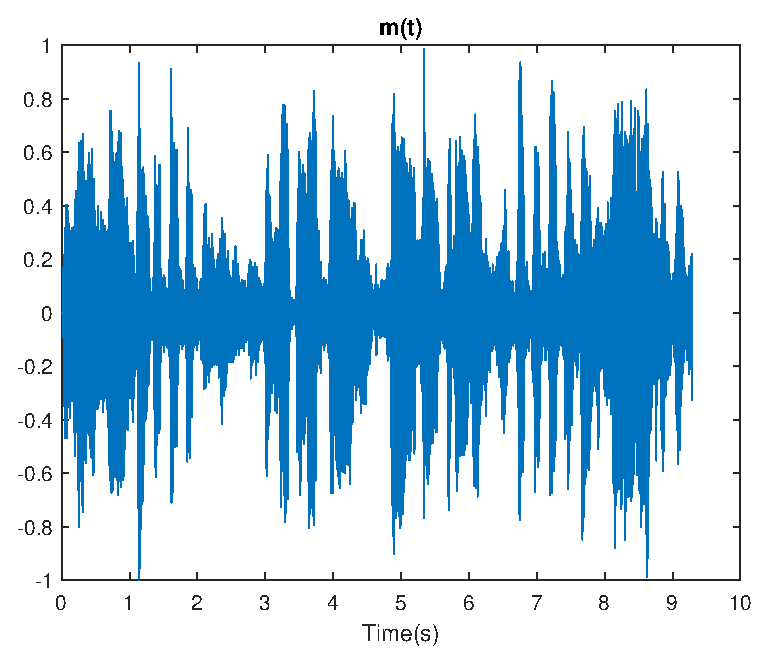
\includegraphics [width=4in]{ECE300_HW2_01.eps}


\subsection*{Question 1}

\begin{par}
take fft, and create wd and f
\end{par} \vspace{1em}
\begin{verbatim}
M = fft(m);
Ms = (fftshift(M)/fs);
wd = linspace(-pi,pi,N);
wdq = linspace(-pi,pi,N*40); % upsampled wd vector
f = wd*fs/(2*pi);
fq = wdq*fsq/(2*pi); % upsampled frequency vector

% Plotting
figure;
subplot(3,1,1);
semilogy(f,abs(Ms));
ylabel('|M(f)|');
xlabel('Frequency(Hz)');
title('Semi-log Magnitude of M(f)');
subplot(3,1,2);
plot(f,abs(Ms));
ylabel('|M(f)|');
xlabel('Frequency(Hz)');
title('Magnitude of M(f)');
subplot(3,1,3);
plot(f,unwrap(angle(Ms)));
ylabel('Radians');
xlabel('Frequency(Hz)');
title('Phase of M(f)');
\end{verbatim}

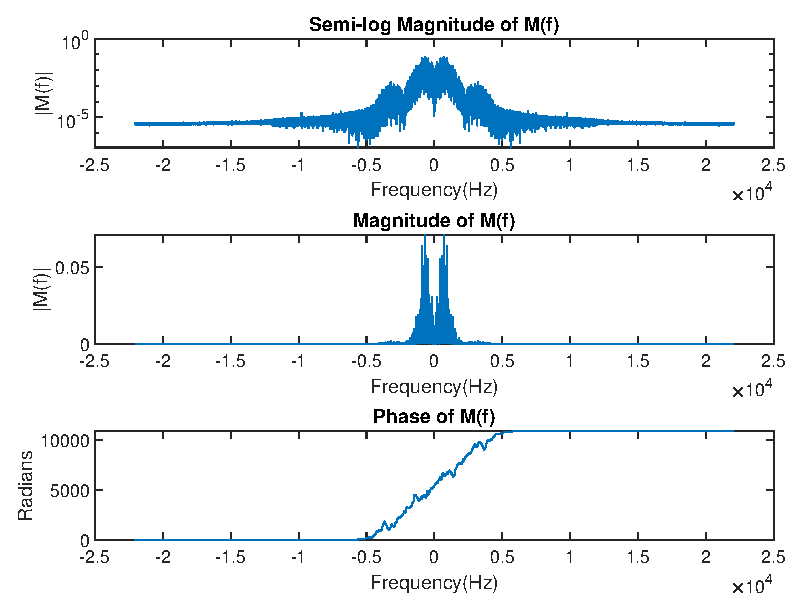
\includegraphics [width=4in]{ECE300_HW2_02.eps}
\begin{par}
The bandwidth of the signal is \ensuremath{\tilde{\;}}4kHz. This was obtained by looking at the positive support of the signal in the frequency domain
\end{par} \vspace{1em}


\subsection*{Question 2}

\begin{verbatim}
fc = 550000; % carrier frequency
c = cos(2*pi*fc*tq);
s = sin(2*pi*fc*tq);
mq = interp1(t,m,tq,'linear','extrap'); % linear interpolated m(t)
\end{verbatim}


\subsection*{Question 3}

\begin{par}
DSC-SC:
\end{par} \vspace{1em}
\begin{verbatim}
u_dsbsc = mq.*c;

% Take fft
U_dsbsc = fft(u_dsbsc);
U_dsbsc_s = (fftshift(U_dsbsc)/fsq);

% Plotting
figure;
subplot(2,2,[1,2]);
plot(tq,u_dsbsc);
xlabel('Time(s)');
title('u_{dsbsc}(t)');
subplot(2,2,3);
semilogy(fq,abs(U_dsbsc_s));
ylabel('log(|U_{dsbsc}|)');
xlabel('Frequency(Hz)');
title('Semi-log Magnitude of U_{dsbsc}(f)');
subplot(2,2,4);
plot(fq,unwrap(angle(U_dsbsc_s)));
ylabel('Radians');
xlabel('Frequency(Hz)');
title('Phase of U_{dsbsc}(f)');
\end{verbatim}

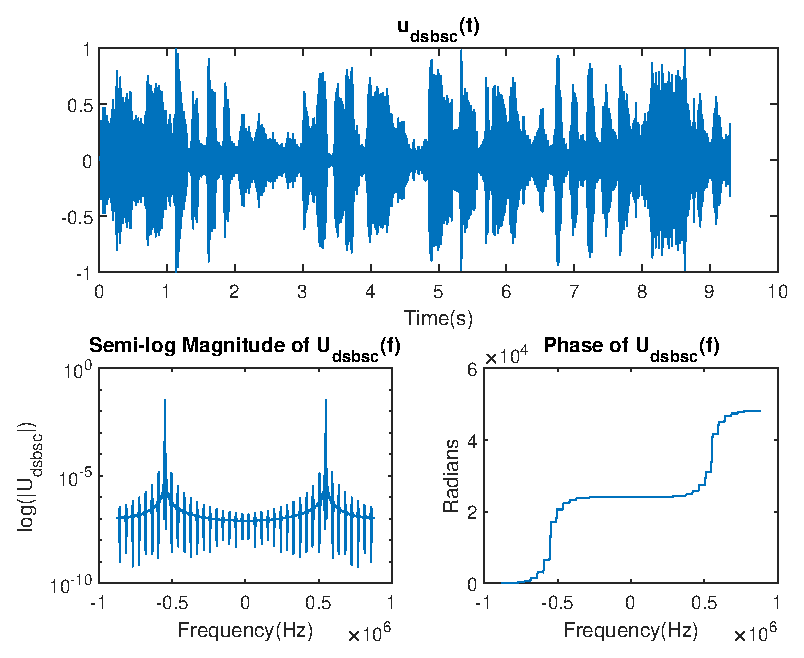
\includegraphics [width=4in]{ECE300_HW2_03.eps}
\begin{par}
DSB-AM:
\end{par} \vspace{1em}
\begin{verbatim}
u_dsb = u_dsbsc + c;

% Take fft
U_dsb = fft(u_dsb);
U_dsb_s = fftshift((U_dsb)/fsq);

% Plotting
figure;
subplot(2,2,[1,2]);
plot(tq,u_dsb);
xlabel('Time(s)');
title('u_{dsb}(t)');
subplot(2,2,3);
semilogy(fq,abs(U_dsb_s));
ylabel('log(|U_{dsb}|)');
xlabel('Frequency(Hz)');
title('Semi-log Magnitude of U_{dsb}(f)');
subplot(2,2,4);
plot(fq,unwrap(angle(U_dsb_s)));
ylabel('Radians');
xlabel('Frequency(Hz)');
title('Phase of U_{dsb}(f)');
\end{verbatim}

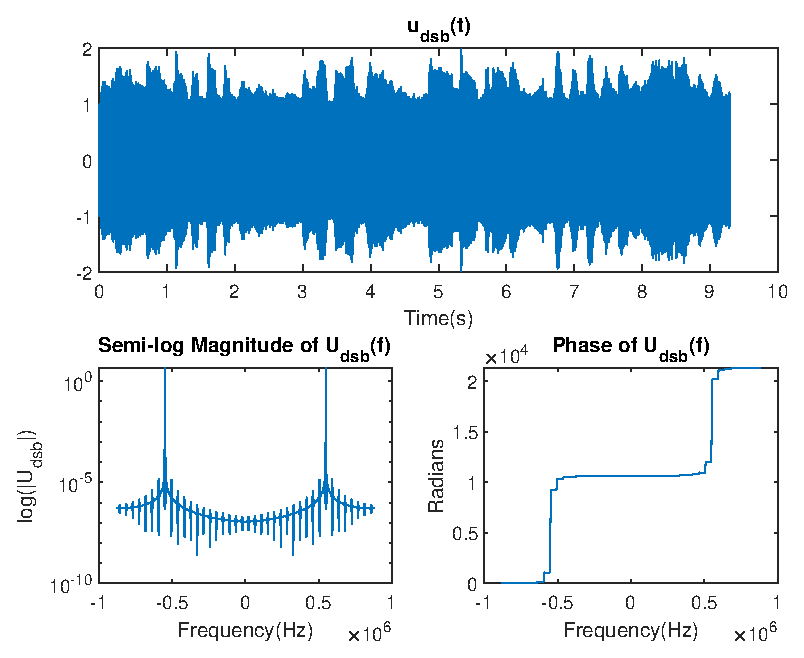
\includegraphics [width=4in]{ECE300_HW2_04.eps}
\begin{par}
The only notable difference between the DSB AM and DSB SC in the frequency domain is that the peak at \ensuremath{\tilde{\;}}550 kHz on the DSB AM is significantly higher than the peak at \ensuremath{\tilde{\;}}550 kHz on the DBS SC.
\end{par} \vspace{1em}


\subsection*{Question 4}

\begin{par}
Upper and Lower SSB AM
\end{par} \vspace{1em}
\begin{verbatim}
u_ussb = mq.*c - HilbertTransform(mq,fq).*s;
u_lssb = mq.*c + HilbertTransform(mq,fq).*s;

% take fft
U_ussb = fft(u_ussb);
U_ussbs = (fftshift(U_ussb)/fs);
U_lssb = fft(u_lssb);
U_lssbs = (fftshift(U_lssb)/fs);

% Plotting
figure;
subplot(3,2,1);
plot(tq,u_ussb);
xlabel('Time(s)');
title('u_{ussb}(t)');
subplot(3,2,2);
plot(tq,u_lssb);
xlabel('Time(s)');
title('u_{lssb}(t)');
subplot(3,2,3);
semilogy(fq,abs(U_ussbs));
ylabel('log(|U_{lssb}|)');
xlabel('Frequency(Hz)');
title('Semi-log Magnitude of U_{ussb}(f)');
subplot(3,2,4);
semilogy(fq,abs(U_lssbs));
ylabel('log(|U_{ussb}|)');
xlabel('Frequency(Hz)');
title('Semi-log Magnitude of U_{lssb}(f)');
subplot(3,2,5);
plot(fq,unwrap(angle(U_ussbs)));
ylabel('Radians');
xlabel('Frequency(Hz)');
title('Phase of U_{ussb}(f)');
subplot(3,2,6);
plot(fq,unwrap(angle(U_lssbs)));
ylabel('Radians');
xlabel('Frequency(Hz)');
title('Phase of U_{lssb}(f)');
\end{verbatim}

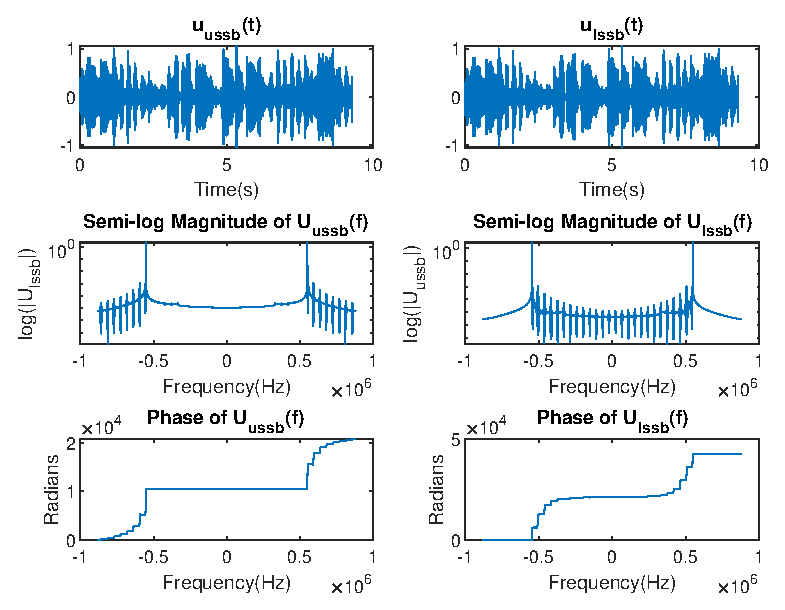
\includegraphics [width=4in]{ECE300_HW2_05.eps}


\subsection*{Question 5}

\begin{par}
Conventional AM
\end{par} \vspace{1em}
\begin{verbatim}
u_conventional = (1+mq).*c;

% Take fft
U_conventional = fft(u_conventional);
U_conventional_s = (fftshift(U_conventional)/fsq);

% Plotting
figure;
subplot(2,2,[1,2]);
plot(tq,u_conventional);
xlabel('Time(s)');
title('u_{conventional}(t)');
subplot(2,2,3);
semilogy(fq,abs(U_conventional_s));
ylabel('log(|U_{conventional}|)');
xlabel('Frequency(Hz)');
title('Semi-log Magnitude of U_{conventional}(f)');
subplot(2,2,4);
plot(fq,unwrap(angle(U_conventional_s)));
ylabel('Radians');
xlabel('Frequency(Hz)');
title('Phase of U_{conventional}(f)');
\end{verbatim}

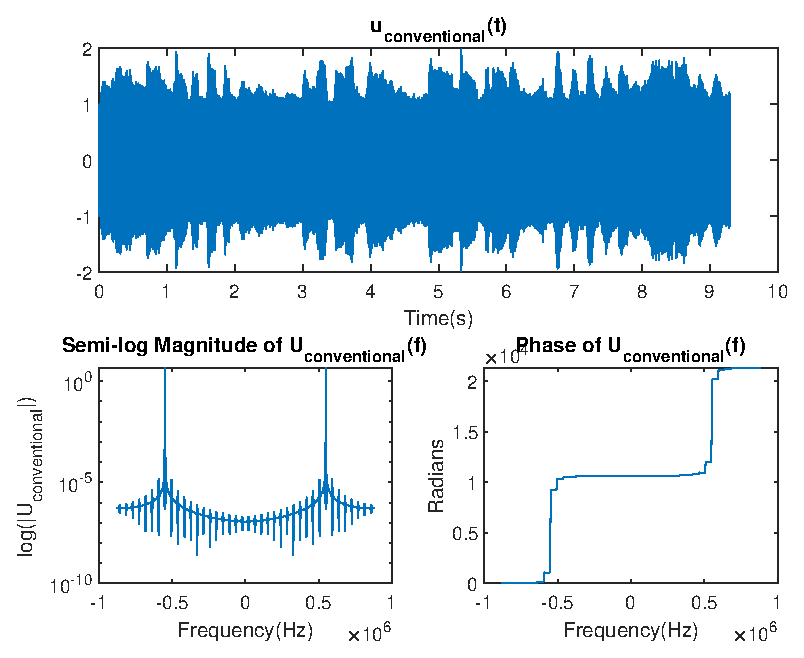
\includegraphics [width=4in]{ECE300_HW2_06.eps}


\subsection*{Question 6}

\begin{par}
Demodulation
\end{par} \vspace{1em}
\begin{verbatim}
% Rectification
u_conventional(u_conventional < 0) = 0;

% Take fft and plot
U_conventional = fft(u_conventional);
U_conventional_s = (fftshift(U_conventional)/fsq);

% Plotting
figure;
subplot(2,2,[1,2]);
plot(tq,u_conventional);
xlabel('Time(s)');
title('u_{conventional}(t) Rectified');
subplot(2,2,3);
semilogy(fq,abs(U_conventional_s));
ylabel('log(|U_{conventional}|)');
xlabel('Frequency (Hz)');
title('Semi-log Magnitude of U_{conventional}(f) Rectified');
subplot(2,2,4);
plot(fq,unwrap(angle(U_conventional_s)));
ylabel('Radians');
xlabel('Frequency(Hz)');
title('Phase of U_{conventional}(f) Rectified');

% Filtering: cutoff of 3kHz gave good sound quality
filter = 2*pi*3000./(abs(fq) + 2*pi*3000); % first order low pass filter
U_filtered = U_conventional_s.*filter; % multiplication in frequency domain
u_filtered = ifft(fftshift(U_filtered)*fsq); % convert back to time domain

% Plotting
figure;
subplot(2,2,[1,2]);
plot(tq,abs(u_filtered));
xlabel('Time(s)');
title('u_{filtered}(t)');
subplot(2,2,3);
semilogy(fq,abs(U_filtered));
ylabel('log(|U_{filtered}|)');
xlabel('Frequency (Hz)');
title('Semi-log Magnitude of U_{filtered}(f)');
subplot(2,2,4);
plot(fq,unwrap(angle(U_filtered)));
ylabel('Radians');
xlabel('Frequency(Hz)');
title('Phase of U_{filtered}(f)');

% downsampling and play sound
u_filtered_downsampled = decimate(u_filtered,40);
sound(real(u_filtered_downsampled),fs);
\end{verbatim}

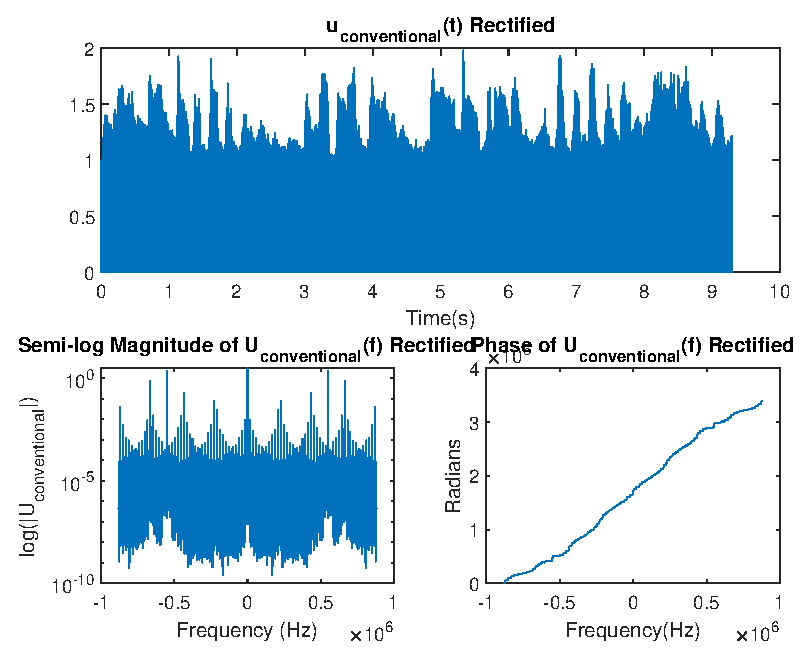
\includegraphics [width=4in]{ECE300_HW2_07.eps}

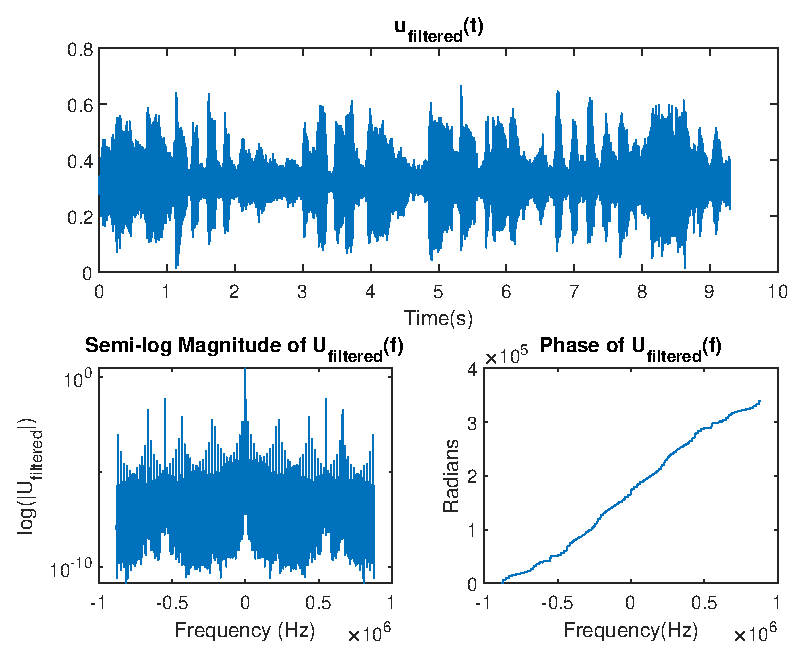
\includegraphics [width=4in]{ECE300_HW2_08.eps}



\end{document}

